\documentclass{article}
\usepackage[a4paper,margin=2.5cm]{geometry} % set A4 paper size and 2.5cm margins
\usepackage{amsmath}
\usepackage{graphicx} % Required for inserting images
\usepackage{subcaption}
\usepackage{hyperref}
\usepackage[backend=biber]{biblatex}
\addbibresource{bibliography.bib}
\hypersetup{
    colorlinks=true,
    linkcolor=black,
    filecolor=black,      
    urlcolor=blue,
    citecolor=black,
    pdftitle={Overleaf Example},
    pdfpagemode=FullScreen,
    }

\title{Machine Learning For Data Science I, \\[0.1cm] Homework 05}

\author{Maj Gaberšček, 27212075}
\date{May 2023}

\begin{document}

\maketitle

\section{Problem}

The problem of this homework was to implement two kernel classes (the polynomial kernel and the RBF kernel) and two regression methods (kernelized ridge regression and support vector regression). 

\section{Implementation}

\subsection{RBF kernel}
This implementation was nothing really special. We set the sigma parameter, when initializing the object. When calling it, we check for \texttt{x} and \texttt{y} dimension and return kernel values.

\subsection{Polynomial kernel}
Again, we set the dimension to the polynomial kernel, when initializing it. Later, when calling it, we firstly check the dimension of the inputs and return correct kernel values.

I also had to add the $\gamma$ parameter for scaling. Otherwise, polynomial kernels could not be combined with SVR (because of some trouble with \texttt{cvxopt.solvers.qp} optimization).

\subsection{Kernelized ridge regression}
When fitting the kernelized ridge regression, we first calculate the kernel matrix, \texttt{K}. Regarding the closed form solution we sets weights as $$w = (K + \lambda I)^{-1} y.$$ When predicting, we calculate $k'x = kernel(X_{train}, X_{predict})$ and dot multiply it with weight matrix.

\subsection{Support vector regression}
When fitting SVR, the main goal is to understand, that we must convert problem in Equation 10 of \cite{smola2004tutorial} to the QP problem, where we are minimizing $\frac{1}{2} x^T P x + q^T x$, subject to $G x <= h$ and $A x = b$. Most challenging was finding a matrix $P$, as instructions stated that $x$ had to be of form $x = [\alpha_1, \alpha_1^*,..., \alpha_n, \alpha_n^*]$. So after some thoughts, I found out, that: $P = p_{ij}$, where $p_{ij}$ is a block of size 2x2: 

\[
p_{ij} = \begin{bmatrix}
\langle x_i, x_j \rangle & -\langle x_i, x_j \rangle \\
-\langle x_i, x_j \rangle & \langle x_i, x_j \rangle
\end{bmatrix}
\]

Other matrices were not that hard to find. After parameter optimization with the help of \texttt{cvxopt.solvers.qp} function, we set alphas and support vectors to the model.

\section{The sine dataset}

Here, the main goal was to find some parameters, for which the method/kernel would perform relatively good. I plotted performance of models (in regard to MSE on training set). I did not include the plots in the report, but they can be found in plots folder on my \href{https://github.com/majbc1999/ml-for-data-science-homeworks} {Github repository}. Of course green color means better performance and red color worse.

So by finding some good parameters, I applied models to the sine dataset, marked the fit, the data and (if the model is SVR) the support vectors (Figures \ref{fig:sine_KRR_polynomial}, \ref{fig:sine_KRR_RBF}, \ref{fig:sine_SVR_polynomial}, \ref{fig:sine_SVR_RBF}). Parameters, that were used for fitting, are printed in the title of every plot. 

\begin{figure}[!h]
    \centering
    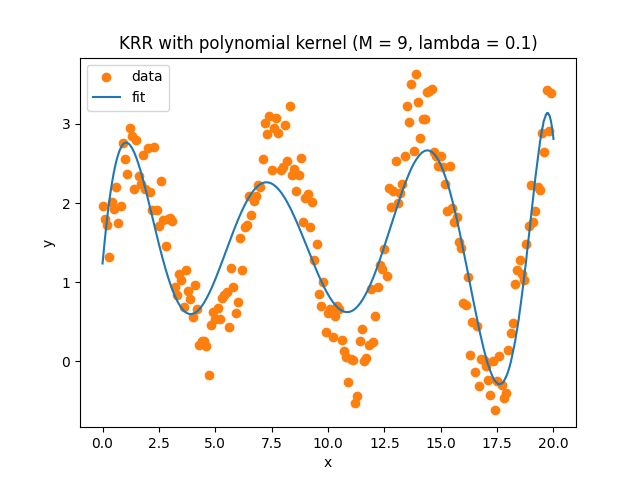
\includegraphics[width=0.5\textwidth]{homework-05/plot/sine_KRR_polynomial.png}
    \caption{The fit and data for kernelized ridge regression with polynomial kernel}
    \label{fig:sine_KRR_polynomial}
\end{figure}

\begin{figure}[!h]
    \centering
    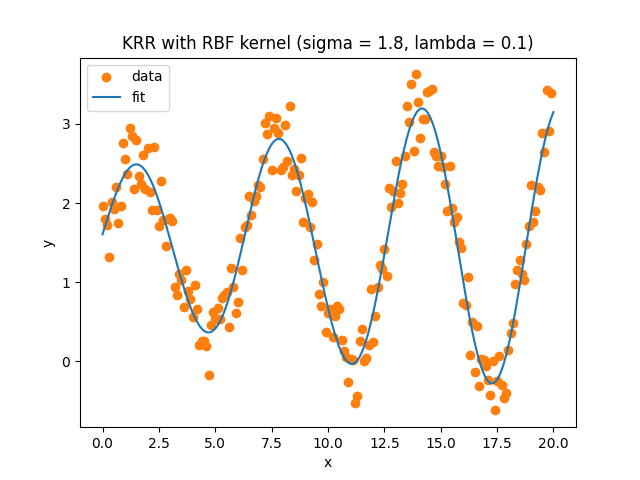
\includegraphics[width=0.5\textwidth]{homework-05/plot/sine_KRR_RBF.png}
    \caption{The fit and data for kernelized ridge regression with RBF kernel}
    \label{fig:sine_KRR_RBF}
\end{figure}

\begin{figure}[!h]
    \centering
    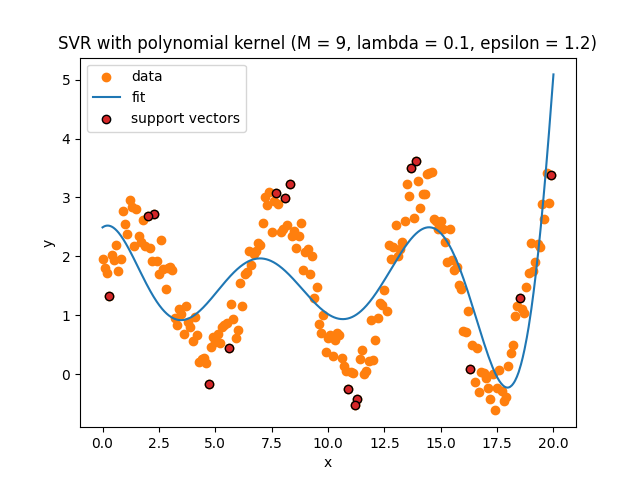
\includegraphics[width=0.5\textwidth]{homework-05/plot/sine_SVR_polynomial.png}
    \caption{The fit and data for SVR with polynomial kernel}
    \label{fig:sine_SVR_polynomial}
\end{figure}

\begin{figure}[!h]
    \centering
    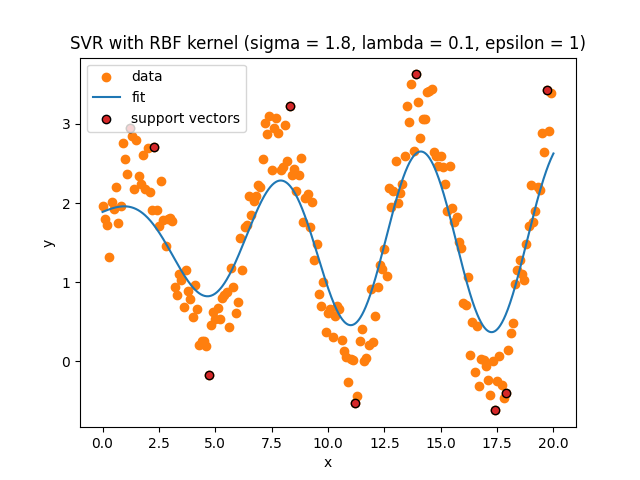
\includegraphics[width=0.5\textwidth]{homework-05/plot/sine_SVR_RBF.png}
    \caption{The fit and data for SVR with RBF kernel}
    \label{fig:sine_SVR_RBF}
\end{figure}

For SVM, I also produced a sparse solution. That is done by checking the weights (more specifically the weight difference $\alpha_i - \alpha_i^*$). If weights are very small, we can exclude the corresponding vector from our prediction.

\section{The housing dataset}

Next, I applied both regression methods with combination of both kernels to the housing dataset. I plotted MSE in regard to $M$ (polynomial kernel) and $\sigma$ (for the RBF kernel). As I didn't really know what values to compare for $sigma$, I decided to use the logarithmic scale. 

One plot was for $\lambda=1$ and the other plot was for optimal $\lambda$, set with internal cross validation. By doing this, we should reduce the risk of overfitting. However, we can still see, that models with $\lambda=1$ sometimes overperform models with optimal $\lambda$, when calculating the MSE on a separating testing set. Plots for MSE can be seen in Figure \ref{fig:comparison}. 

\begin{figure}[!h]
    \centering
    
    \begin{subfigure}[b]{0.45\textwidth}
        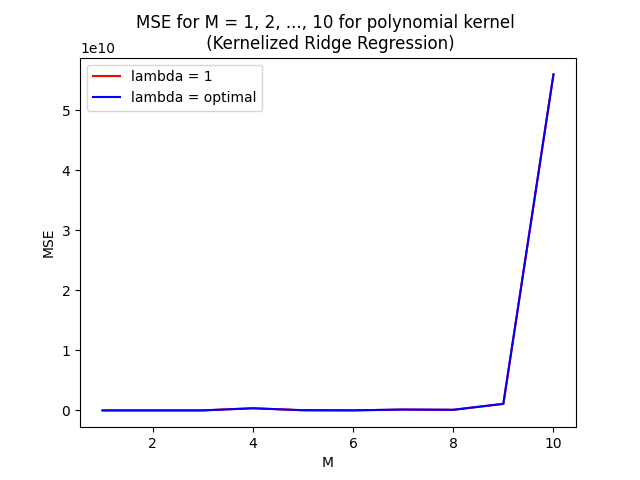
\includegraphics[width=\textwidth]{homework-05/plot/mse_comparison1.png}
    \end{subfigure}
    \hfill
    \begin{subfigure}[b]{0.45\textwidth}
        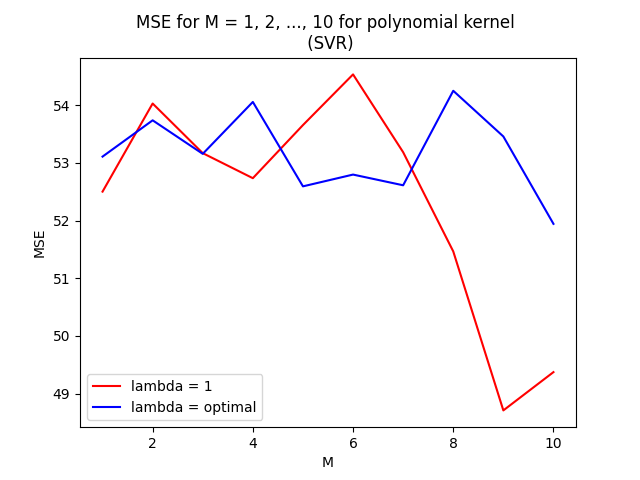
\includegraphics[width=\textwidth]{homework-05/plot/mse_comparison2.png}
    \end{subfigure}
    
    \vspace{0.5cm}
    
    \begin{subfigure}[b]{0.45\textwidth}
        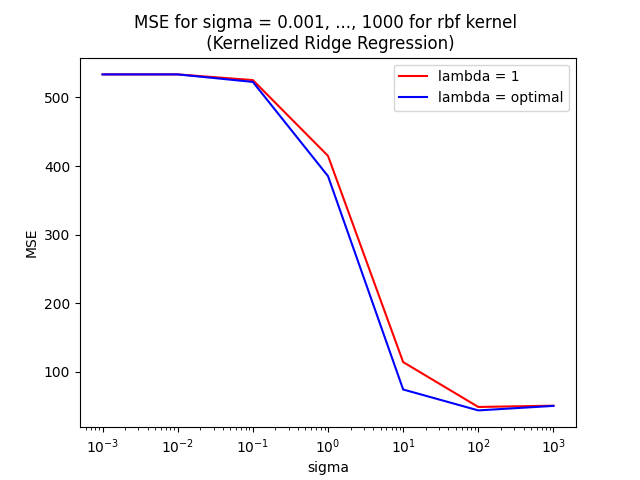
\includegraphics[width=\textwidth]{homework-05/plot/mse_comparison3.png}
    \end{subfigure}
    \hfill
    \begin{subfigure}[b]{0.45\textwidth}
        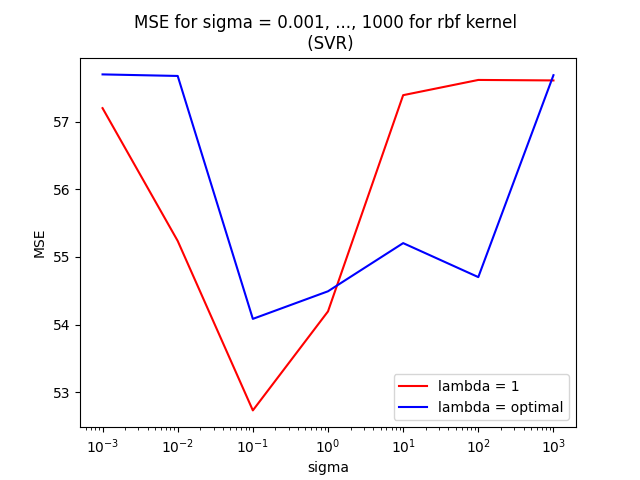
\includegraphics[width=\textwidth]{homework-05/plot/mse_comparison4.png}
    \end{subfigure}
    
    \caption{MSE on the test set in regard to parameters}
    \label{fig:comparison}
\end{figure}

For support vector regression, I also checked how number of vectors included affect the MSE. I plotted how MSE changes in regard to number of support vectors for both kernels and all parameters. I filtered out vectors one by one, first those, whose weight was the smallest and so on. I did not include all the visualizations in my report. Again, they are included in my \href{https://github.com/majbc1999/ml-for-data-science-homeworks} {Github repository}. Just to paint a picture, I am including two samples in Figures \ref{fig:SVR_number1} and \ref{fig:SVR_number2}. We can see, that it would be safe to take 70 vectors (in first example) and around 90 vectors (in the second example).

\begin{figure}[!h]
    \centering
    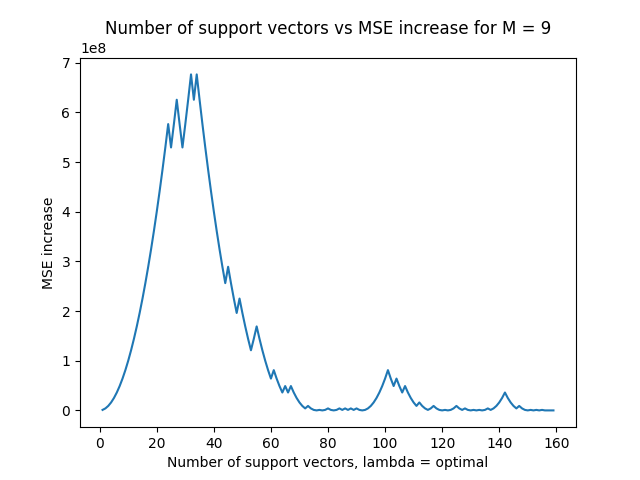
\includegraphics[width=0.8\textwidth]{homework-05/plot/number_of_vectors_9-opt.png}
    \caption{Percentual MSE increase in regard to support vector number, polynomial kernel with $M = 9$ and optimal $\lambda$}
    \label{fig:SVR_number1}
\end{figure}

\begin{figure}[!h]
    \centering
    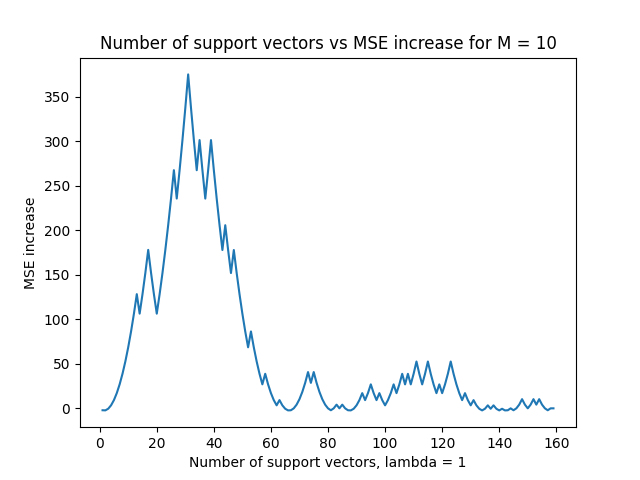
\includegraphics[width=0.8\textwidth]{homework-05/plot/number_of_vectors_10-1.png}
    \caption{Percentual MSE increase in regard to support vector number, RBF kernel with $\sigma = 10$ and optimal $\lambda$}
    \label{fig:SVR_number2}
\end{figure}

\section{Conclusions}
As we can see in the sine dataset, the kernelized ridge regression was able to predict the fit better (more accurately). However, when computing the model on the housing dataset, SVR proved to be more stable. For example, the kernelized ridge regression in combination with polynomial kernel generated MSEs of great magnitude. 

Regarding my preferences, I prefered the kernelized ridge regression, simply for the fact, that I did not need to use additional libraries and packages for optimization.

\printbibliography

\end{document}